%
% $RCSfile: article.tex,v $
%
% Copyright (c) 2001-2002. Christian Heller. All rights reserved.
%
% No copying, altering, distribution or any other actions concerning this
% document, except after explicit permission by the author!
% At some later point in time, this document is planned to be put under
% the GNU FDL license. For now, _everything_ is _restricted_ by the author.
%
% http://www.resmedicinae.org
% - Information in Medicine -
%
% @author Christian Heller <christian.heller@tuxtax.de>
%

%
% The document class specifying the type of document.
%
\documentclass[a4paper,10pt]{llncs}

%
% The usepackages for document class.
%

% Paper format and font.
\usepackage{a4,times,helvet}

% Graphics.
\usepackage{graphicx}

%
% The space settings for edges (left, top, right, bottom).
%
\setlength{\hoffset}{-1,3in}
\setlength{\voffset}{-1in}
\setlength{\oddsidemargin}{3,5cm}
\setlength{\topmargin}{1,3cm}
%\setlength{\headwidth}{16,5cm}
\setlength{\headheight}{0cm}
\setlength{\textwidth}{16,5cm}
\setlength{\textheight}{23,2cm}

%
% The hyphenation list.
%
%
% $RCSfile: hyphenation.tex,v $
%
% Copyright (c) 2002-2007. Christian Heller. All rights reserved.
%
% Permission is granted to copy, distribute and/or modify this document
% under the terms of the GNU Free Documentation License, Version 1.1 or
% any later version published by the Free Software Foundation; with no
% Invariant Sections, with no Front-Cover Texts and with no Back-Cover
% Texts. A copy of the license is included in the section entitled
% "GNU Free Documentation License".
%
% http://www.cybop.net
% - Cybernetics Oriented Programming -
%
% Version: $Revision: 1.2 $ $Date: 2007-08-01 13:59:00 $ $Author: christian $
% Authors: Christian Heller <christian.heller@tuxtax.de>
%

\hyphenation{abs-trac-tion}
\hyphenation{ac-tu-ally}
\hyphenation{ana-lyst}
\hyphenation{ana-ly-sis}
\hyphenation{an-cient}
\hyphenation{ap-pli-ca-tion}
\hyphenation{aris-to-tle}
\hyphenation{at-tri-bute}
\hyphenation{be-ing}
\hyphenation{ca-te-go-ri-za-tion}
\hyphenation{client}
\hyphenation{com-po-nen-ti-za-tion}
\hyphenation{com-pu-ter}
\hyphenation{con-fi-gure}
\hyphenation{con-nec-ted}
\hyphenation{cy-ber-ne-tics}
\hyphenation{cyboi}
\hyphenation{cybol}
\hyphenation{cybop}
\hyphenation{des-cribed}
\hyphenation{de-sign}
\hyphenation{de-ve-lop-ment}
\hyphenation{dis-crete}
\hyphenation{di-vide}
\hyphenation{do-main}
\hyphenation{dy-na-mic}
\hyphenation{eli-mi-nate}
\hyphenation{eli-mi-nates}
\hyphenation{eli-mi-na-tion}
\hyphenation{en-gi-nee-ring}
\hyphenation{en-vi-ron-ment}
\hyphenation{ex-pert}
\hyphenation{fi-gure}
\hyphenation{fle-xi-bi-li-sie-rung}
\hyphenation{fun-da-men-tal}
\hyphenation{hard-ware}
\hyphenation{hu-man}
\hyphenation{im-ple-men-ta-tion}
\hyphenation{in-he-rit}
\hyphenation{in-he-ri-tance}
\hyphenation{in-ter-pre-ter}
\hyphenation{java}
\hyphenation{know-ledge}
\hyphenation{lan-guage}
\hyphenation{li-ving}
\hyphenation{lo-gi-cal}
\hyphenation{ma-na-ge-ment}
\hyphenation{mea-ning-ful}
\hyphenation{me-cha-nism}
\hyphenation{me-mo-ry}
\hyphenation{me-thod}
\hyphenation{me-thods}
\hyphenation{mo-del-ling}
\hyphenation{na-ture}
\hyphenation{net-work}
\hyphenation{neu-ral}
\hyphenation{neu-ron}
\hyphenation{ne-ver-en-ding-ly}
\hyphenation{open}
\hyphenation{operating}
\hyphenation{ori-en-ted}
\hyphenation{over-come}
\hyphenation{par-ti-cu-lar}
\hyphenation{prin-ci-ple}
\hyphenation{pro-ba-bi-lis-tic}
\hyphenation{pro-ble-ma-tic}
\hyphenation{pro-gram-ming}
\hyphenation{res-pon-sible}
\hyphenation{re-u-sa-bi-li-ty}
\hyphenation{sci-ence}
\hyphenation{server}
\hyphenation{si-mi-lar}
\hyphenation{soft-ware}
\hyphenation{source}
\hyphenation{spe-cia-li-za-tion}
\hyphenation{spe-ci-fied}
\hyphenation{sta-tic}
\hyphenation{sta-ti-cally}
\hyphenation{sto-chas-tic}
\hyphenation{stone-on-stone}
\hyphenation{struc-ture}
\hyphenation{strug-gling}
\hyphenation{subs-ti-tu-ting}
\hyphenation{su-per-flu-ous}
\hyphenation{sup-ply-ing}
\hyphenation{sys-tem}
\hyphenation{taeu-schungs-ver-such}
\hyphenation{temp-lates}
\hyphenation{tes-ting}
\hyphenation{thin-king}
\hyphenation{un-en-li-vened}
\hyphenation{un-sa-tis-fy-ing}
\hyphenation{va-ry-ing}
\hyphenation{weigh-ted}
\hyphenation{zu-kunfts-si-che-re}


%
% This document is a scientific paper to be handed in for a conference.
%
% @version 0.1.2.0 16.05.2002
% @author Christian Heller <christian.heller@tuxtax.de>
% @author Christian Heller <christian.heller@tu-ilmenau.de>
%
\begin{document}
\twocolumn

\title{An extended Component Lifecycle}
\author{Christian Heller\\
\(<\)christian.heller@tu-ilmenau.de\(>\)}
\institute{Technical University of Ilmenau\\
Faculty for Computer Science and Automation\\
Institute for Theoretical and Technical Informatics\\
PF 100565, Max-Planck-Ring 14, 98693 Ilmenau, Germany\\
http://www.tu-ilmenau.de, fon: +49-(0)3677-69-1230, fax: +49-(0)3677-69-1220 \vspace*{0.5cm}}
\maketitle
\bigskip

\begin{small}
\textbf{Abstract.}
Based on latest achievements in the field of \emph{Component Based Design (CBD)} and
\emph{Component Oriented Programming (COP)}, this article shows how a component
lifecycle can be extended.
The well-known \emph{Hierarchical Model View Controller (HMVC)} design pattern is
considered for the identification of the two concerns \emph{Showable} and \emph{Loadable}
Following, these two concerns are added to a component to demonstrate the
lifecycle extension.
The component framework \emph{ResMedLib} is introduced to show how such communication
between components happens through well-defined interfaces.
A summarizing reflection on the pros and cons of \emph{Aspects} versus \emph{Concerns}
of a component will finalize the article.
\end{small}
\bigskip

\begin{small}
\textbf{Keywords.}
Component Lifecycle, Design Pattern, HMVC, Concern, Aspect, Res Medicinae, ResMedLib
\end{small}

%
% The introduction section.
%
\section{Introduction}

By following \emph{Component Based Design (CBD)} rules, software projects try to integrate
most diverse systems into one environment. Although the systems should ideally use
\emph{Component Oriented Programming (COP)} for the implementation of their components,
this is not a must. Legacy systems can be encapsulated as well \cite{brown},
acting as one component to the outside environment.
In practice, one cannot use COP without first designing with components in mind.
A typical component oriented development process is displayed in Figure
\ref{fig:component_oriented_development}.

\begin{figure}[ht]
\begin{center}
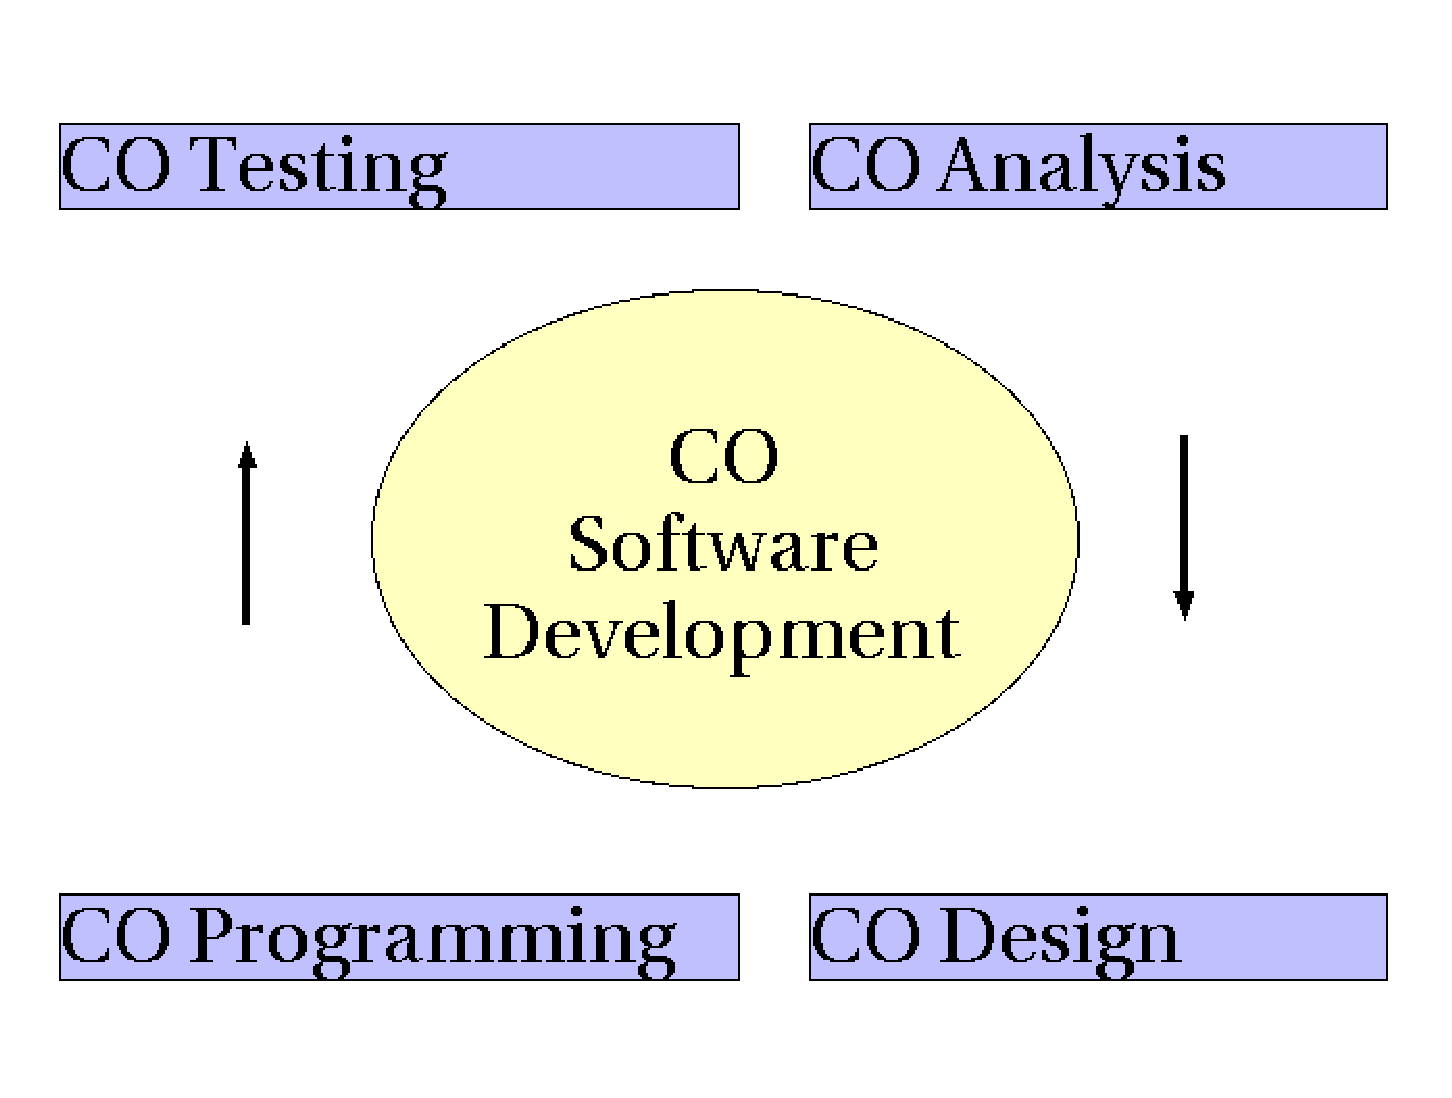
\includegraphics[scale=0.3]{component_oriented_development}
\caption{Component Oriented Software Development.}
\label{fig:component_oriented_development}
\end{center}
\end{figure}

Each component lives in a system that is responsible for the component's
creation, destruction etc. This is to be the topic of this article.
What will not be considered, is the communication between remote components
living in different systems (RMI, CORBA, SOAP) \cite{blueprints} or processes (JMS).\\
When talking about components, this article sticks to the definition of \cite{jakarta}
which considers components to be "a passive entity that performs a specific role".
This is opposed to active components like \emph{Agents} are.
For each role, its \emph{Interface} has to be specified to the rest of the
system as shown in Figure \ref{fig:communication_between_components}.

\begin{figure}[ht]
\begin{center}
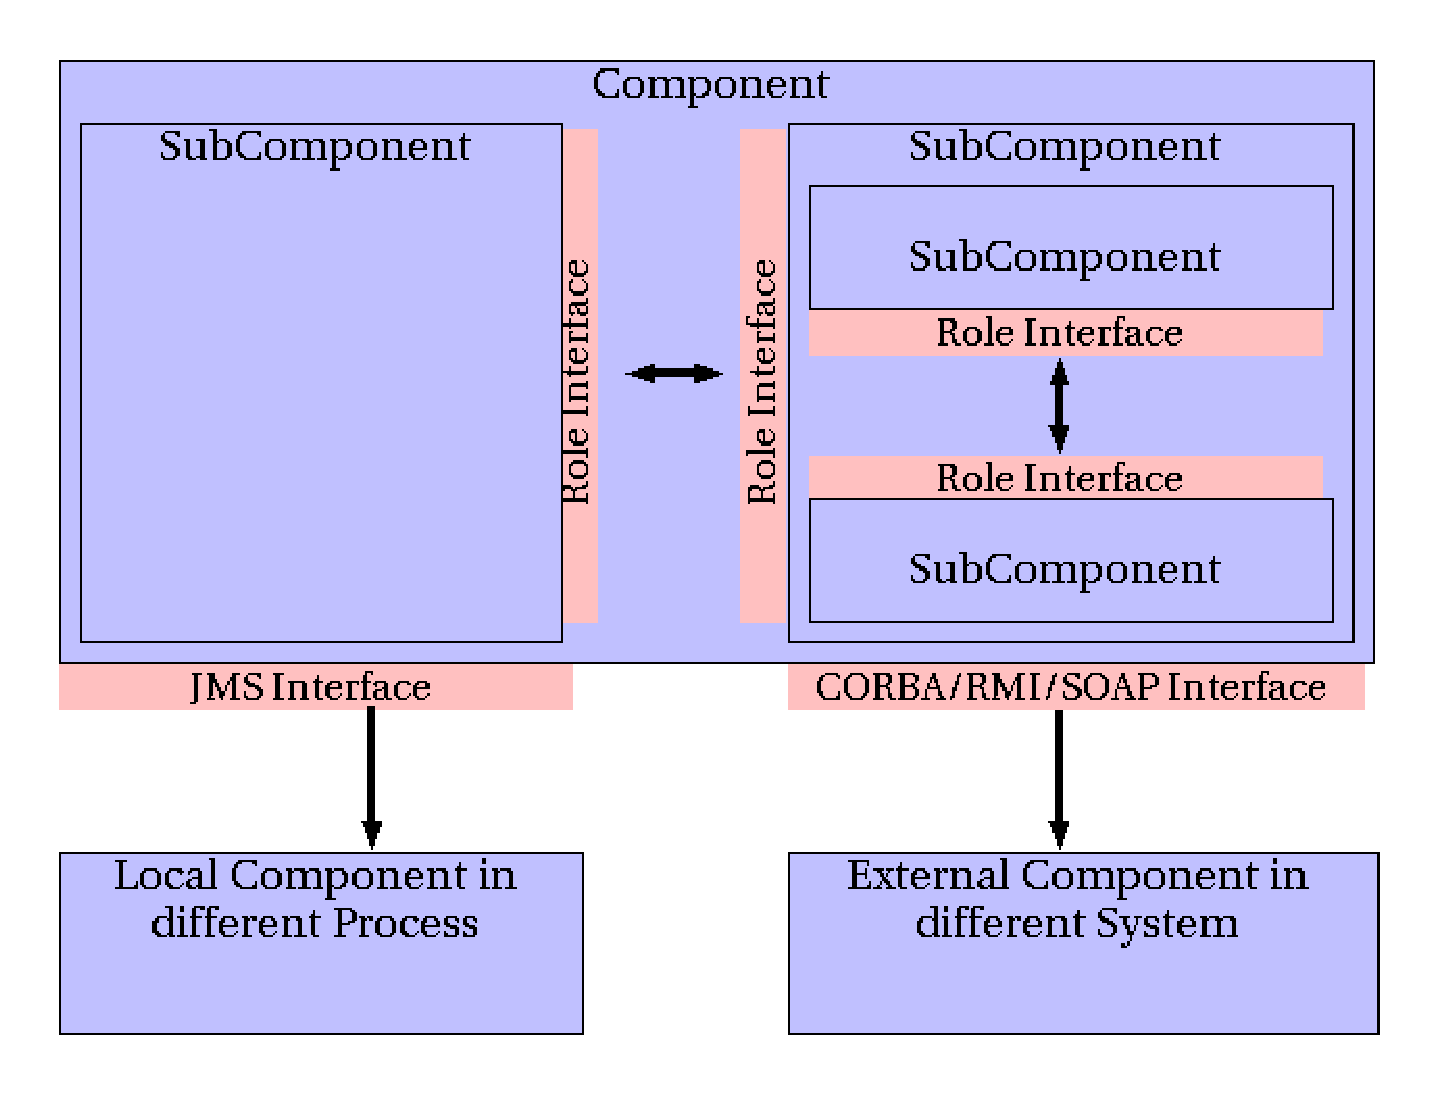
\includegraphics[scale=0.2]{communication_between_components}
\caption{Communication between Components.}
\label{fig:communication_between_components}
\end{center}
\end{figure}

The \emph{Avalon} project \cite{jakarta} writes on to this:
\begin{quotation}
"... the interface is not enough. There are specific
contracts that one must define and keep in mind when specifying the interfaces.
In other words, what users of the component must provide, and what the component
produces. When the interface and contract are defined, one can start to work on
the implementation."
\end{quotation}
As can be seen, there are other concerns besides the component's role (Figure
\ref{fig:role_and_contract_concerns}). In most cases, these concerns belong
to a contract that is defined by the surrounding Framework.

\begin{figure}[ht]
\begin{center}
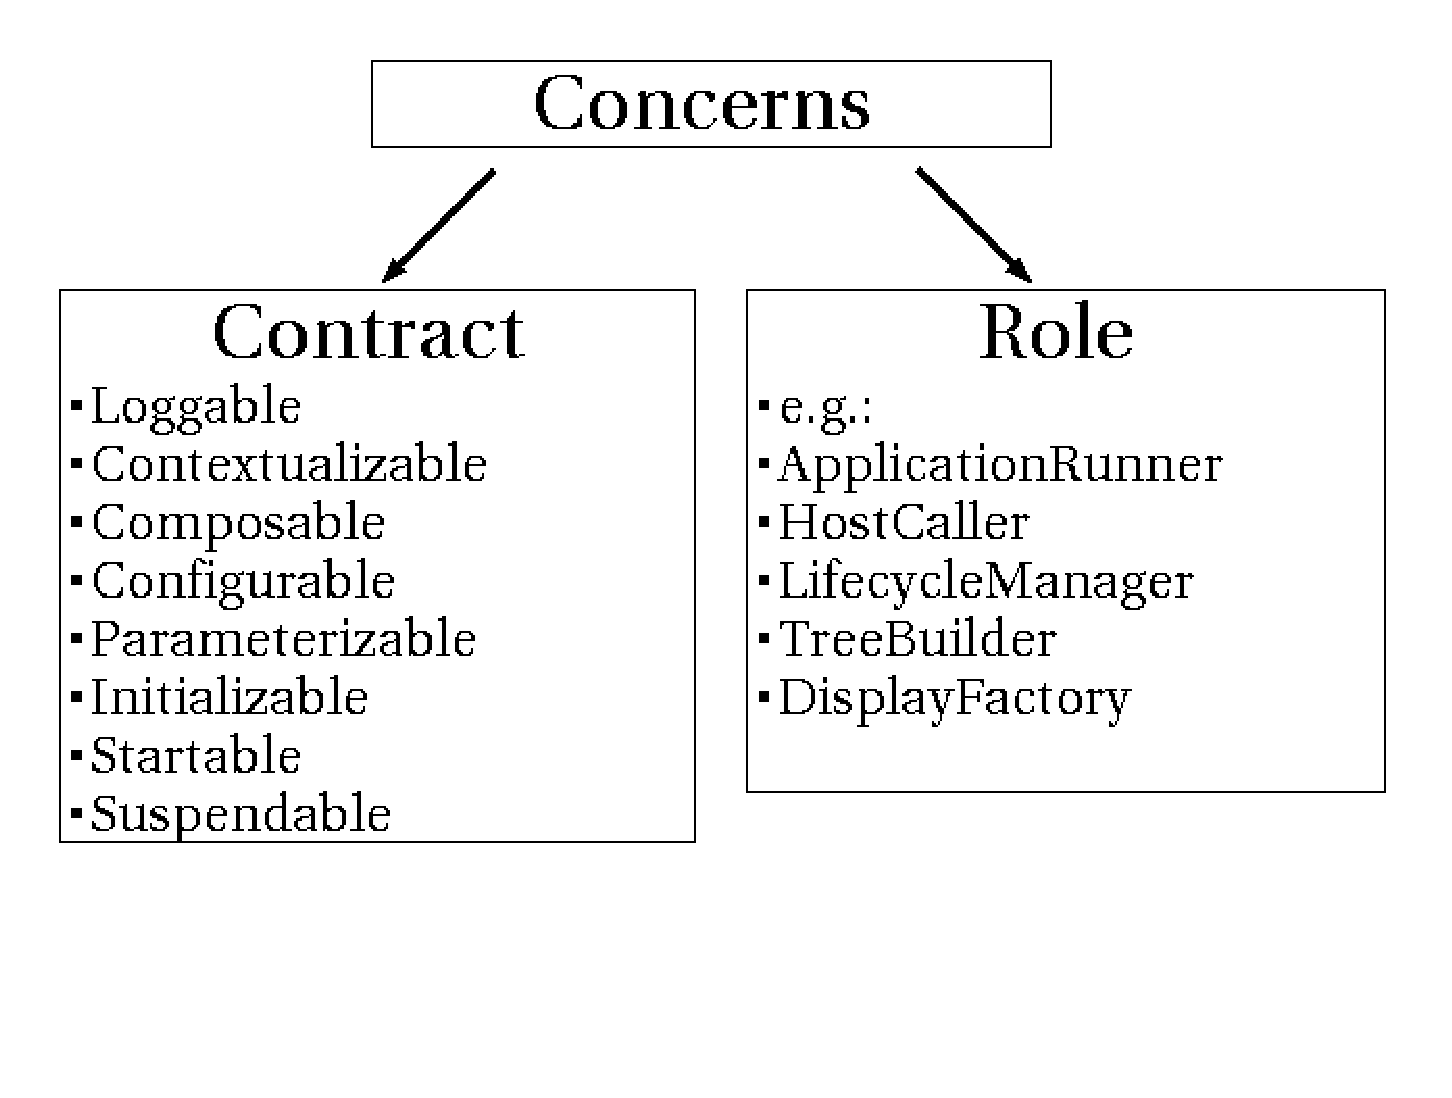
\includegraphics[scale=0.3]{role_and_contract_concerns}
\caption{Role and Contract Concerns.}
\label{fig:role_and_contract_concerns}
\end{center}
\end{figure}

In some way, \emph{Concerns} are quite similar to \emph{Aspects}. In fact,
aspects also provide various outside views (interfaces) to a component (module).
The \emph{AspectJ} project \cite{aspectj} writes:
\begin{quotation}
"Consider what \emph{Aspect Oriented Programming (AOP)} really does:
It makes the modules in a program correspond to modules in the design.
In any given design, some modules are optional, and some are not."
\end{quotation}

They distinguish between \emph{Development} and \emph{Production} aspects
(Figure \ref{fig:possible_systematics_of_concerns_and_aspects}).
Production aspects would be delivered with the finished product, while development aspects
would be used during the development process. Often, production aspects are also
used during development.

\begin{figure}[ht]
\begin{center}
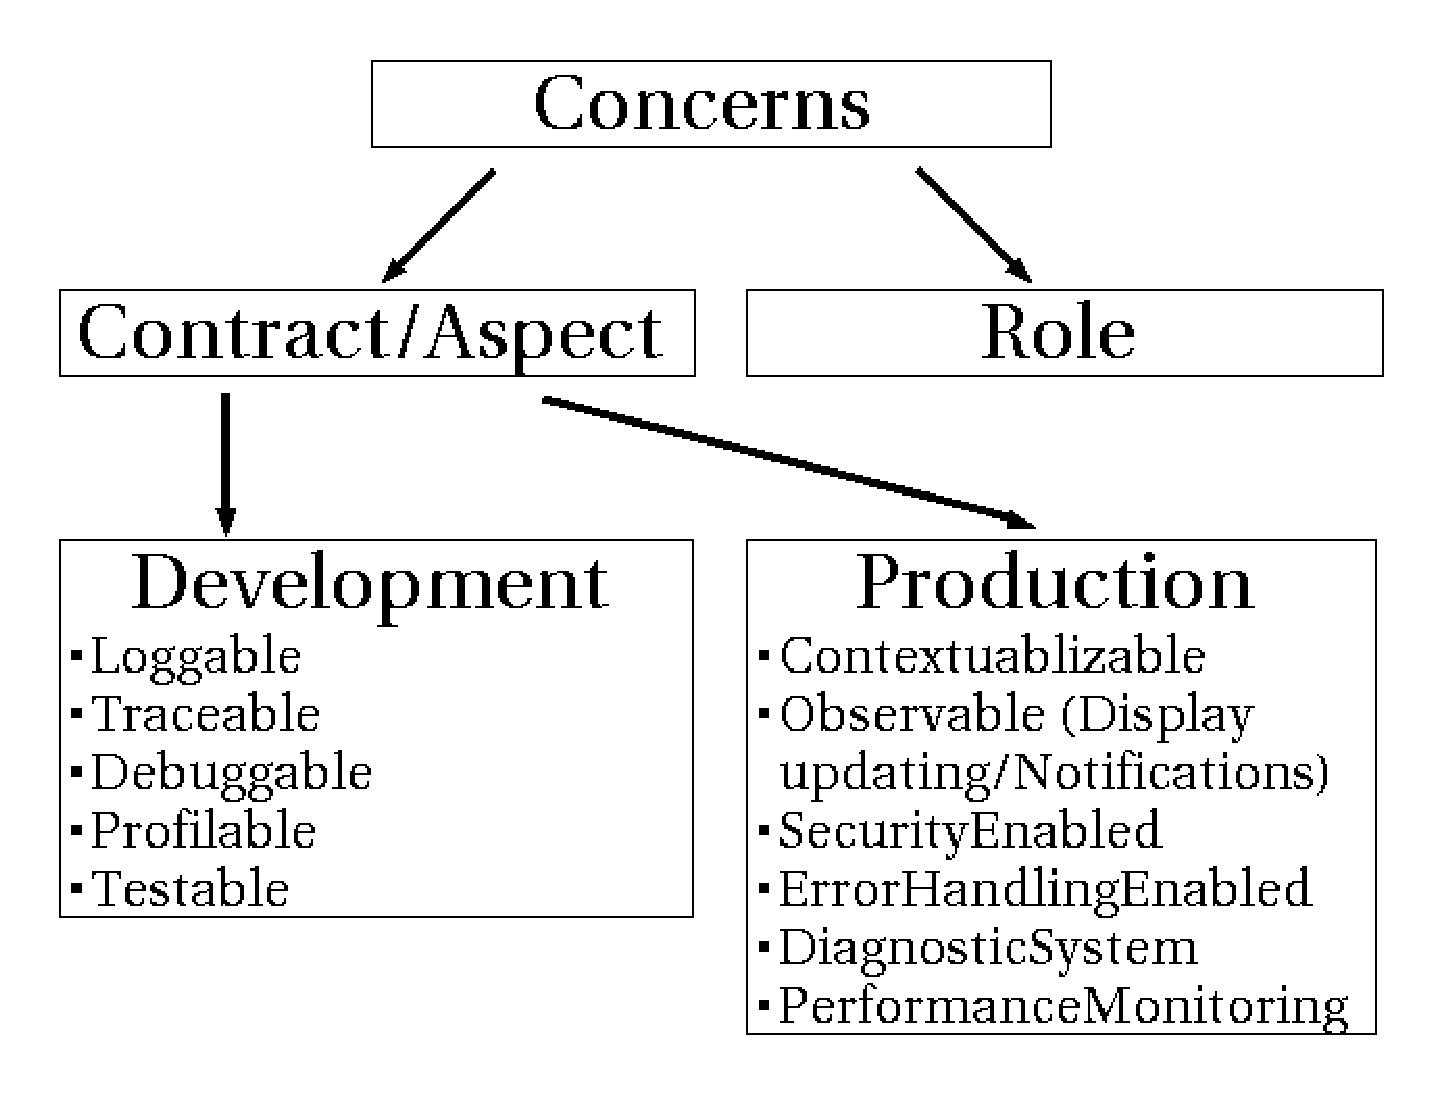
\includegraphics[scale=0.3]{possible_systematics_of_concerns_and_aspects}
\caption{Possible Systematics of Concerns and Aspects.}
\label{fig:possible_systematics_of_concerns_and_aspects}
\end{center}
\end{figure}

Common development aspects are used for logging, tracing, debugging, profiling
or testing. Common production aspects are used for performance monitoring and
diagnostic systems, for display updating or notifications in general, for
security, context passing and error handling.

%
% The basics section.
%
\section{Basics}
\subsection{A Component Lifecycle}

As latest research shows, it is highly desirable for nearly all components,
even for simple objects, to implement interfaces (concerns)
(Figure \ref{fig:lifecycle_interfaces_concerns_avalon})
whose methods can be called according to a given order (contract).
Each interface represents a narrow view of the component or object being controlled.
The order of method calls is what is known as \emph{Component Lifecycle}
(Figure \ref{fig:a_component_lifecycle_avalon}).

\begin{figure}[ht]
\begin{center}
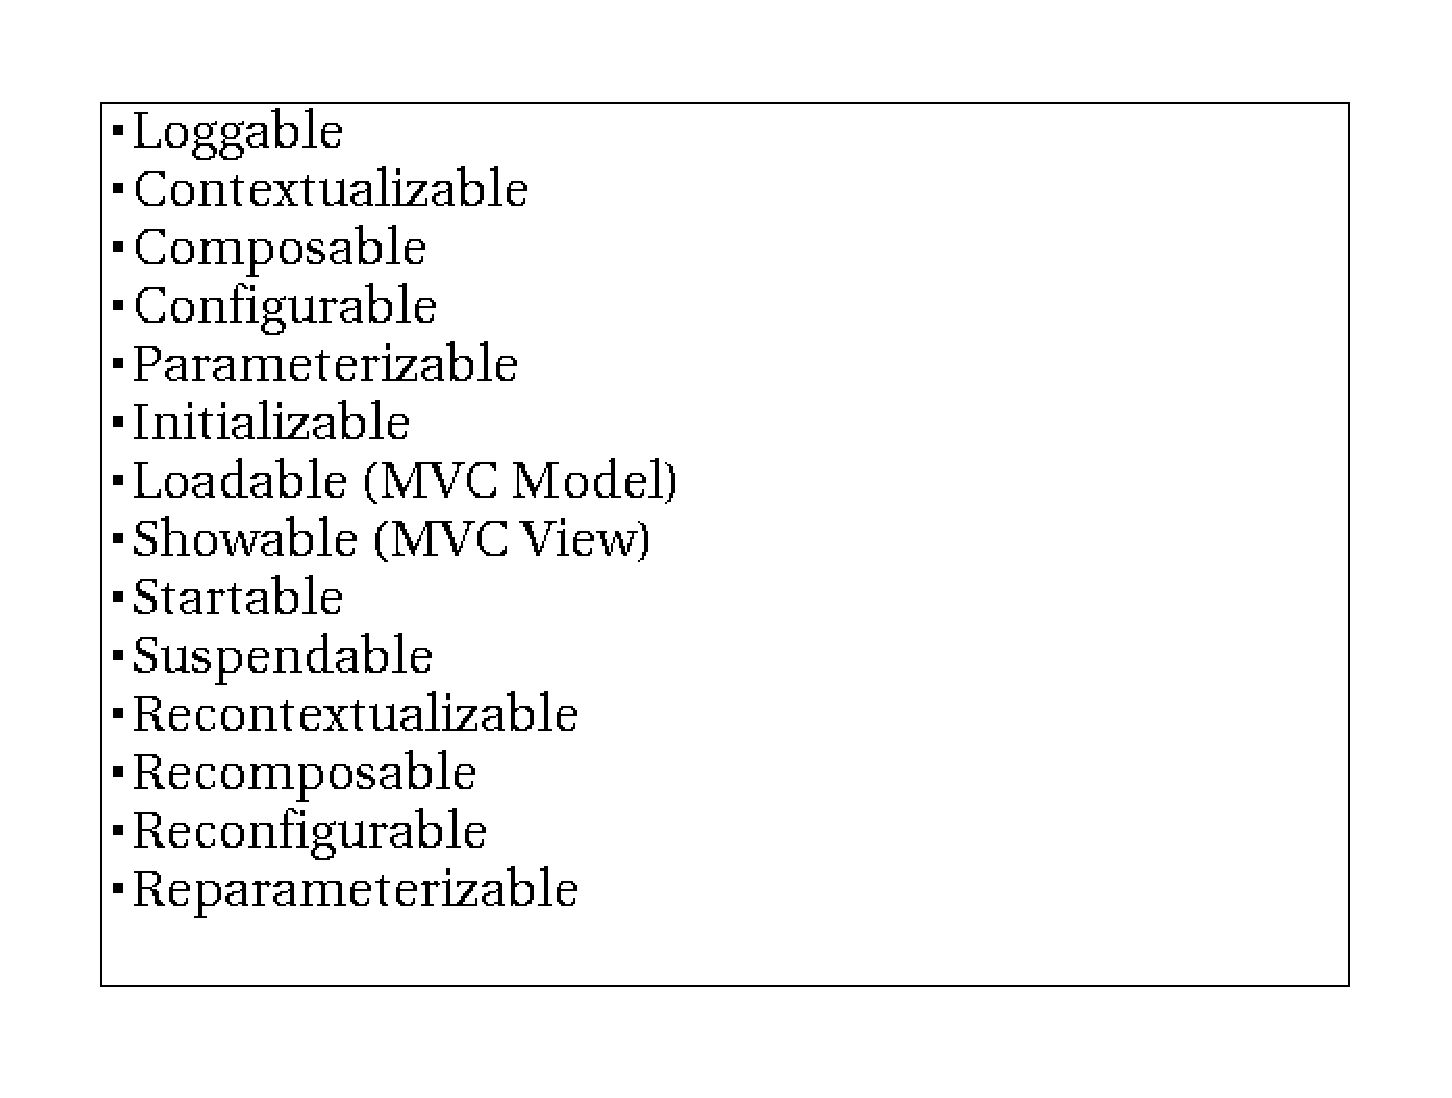
\includegraphics[scale=0.3]{lifecycle_interfaces_concerns_avalon}
\caption{Lifecycle Interfaces/Concerns \cite{jakarta}.}
\label{fig:lifecycle_interfaces_concerns_avalon}
\end{center}
\end{figure}

\begin{figure}[ht]
\begin{center}
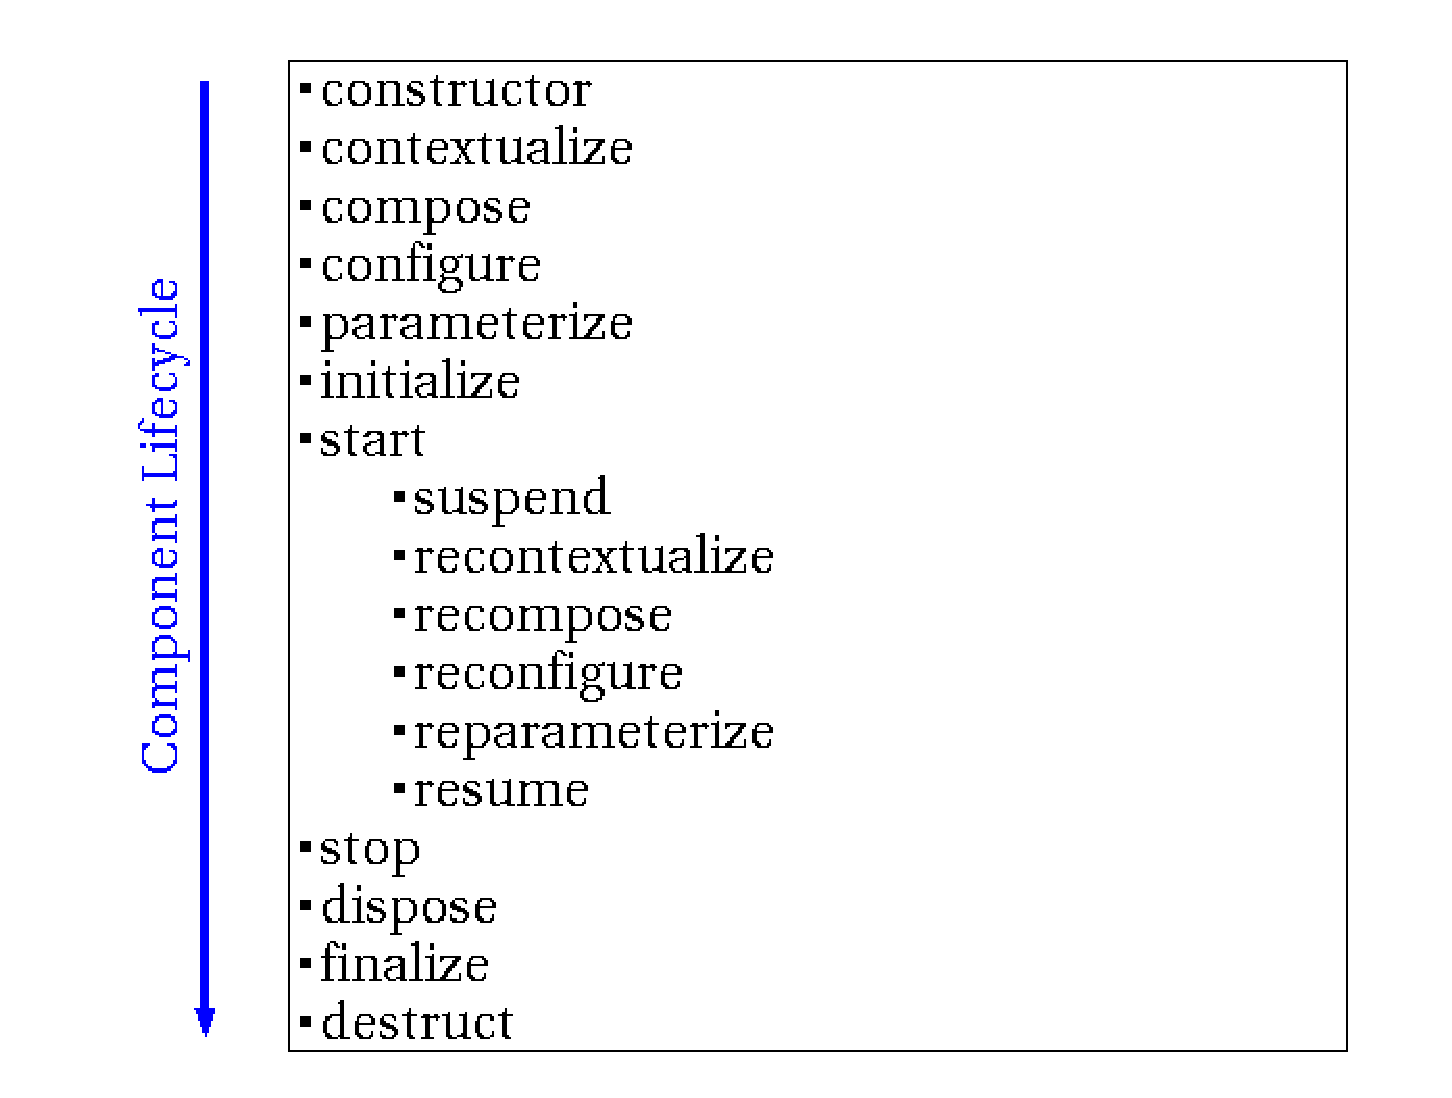
\includegraphics[scale=0.3]{a_component_lifecycle_avalon}
\caption{A Component Lifecycle \cite{jakarta}.}
\label{fig:a_component_lifecycle_avalon}
\end{center}
\end{figure}

An outside, active entity is responsible for calling the component lifecycle
methods in the right order. Such an entity or \emph{Component Container} implements
the \emph{Composable} interface and such controls and uses components.
Avalon \cite{jakarta}: "It is up to each container to indicate which lifecycle methods it will honor.
This should be clearly documented together with the description of the container."

\subsection{The HMVC Design Pattern}

It is - or, at least, should be - a common standard to use a \emph{Model-View-Controller (MVC)}
separation for the \emph{Application} (sometimes called \emph{Presentation}) \emph{Layer} of a system.
The advantages are at hand: A clear encapsulation of code makes it modular and easily exchangeable.
Unnecessary dependencies are avoided and the system layers get decoupled.

Such flexibility allows for the introduction of changeable system parts, for the \emph{View} as well as
for the \emph{Model}. The view, for example, might be switchable between a web frontend based on
\emph{Java Server Pages (JSP)} and a standalone \emph{Graphical User Interface (GUI)} based on \emph{Swing}.
The data sources of a model, on the other hand, might be switchable between File, DB, CORBA/SOAP/RMI,
which together comes close to a complete persistence layer.

\begin{figure}[ht]
\begin{center}
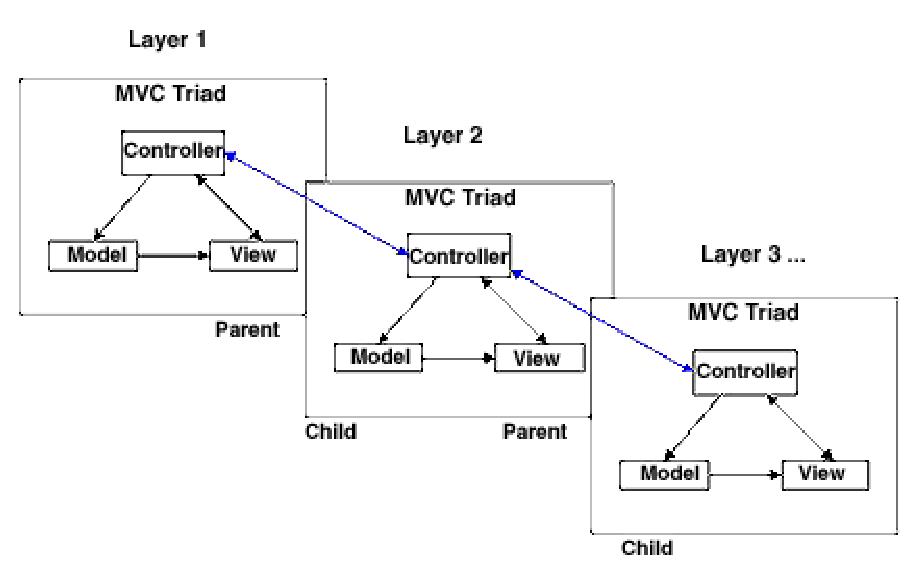
\includegraphics[scale=0.4]{mvc_layers_cai}
\caption{MVC Layers \cite{cai}.}
\label{fig:mvc_layers_cai}
\end{center}
\end{figure}

The MVC \cite{fowler2002} was extended by \cite{cai}
to the \emph{Hierarchical MVC (HMVC)} pattern [Figure \ref{fig:mvc_layers_cai}].
The new idea of HMVC is to have controllers coordinating the process
flow while organizing the communication between view and model.
A second core idea is to allow controllers to have children.
In such a manner, the hierarchy of controllers (\emph{MVC Triads}) represents the
backbone of a system whose startable root controller is called an \emph{Application}.

Child controllers (Figure \ref{fig:hmvc_client_tier_instance_diagram_cai})
should be introduced for \emph{Frames}/\emph{Dialogs}, \emph{Panels} or smaller GUI components,
when the controlling code gets too large. For example, a \emph{Tree} or \emph{Table} GUI component
may become quite complex and require an own controller. However, it is not a must to create many child controllers.
GUI components/panels/dialogs etc. which have no very own controller, will simply
be controlled by the next higher parent controller.

\begin{figure}[ht]
\begin{center}
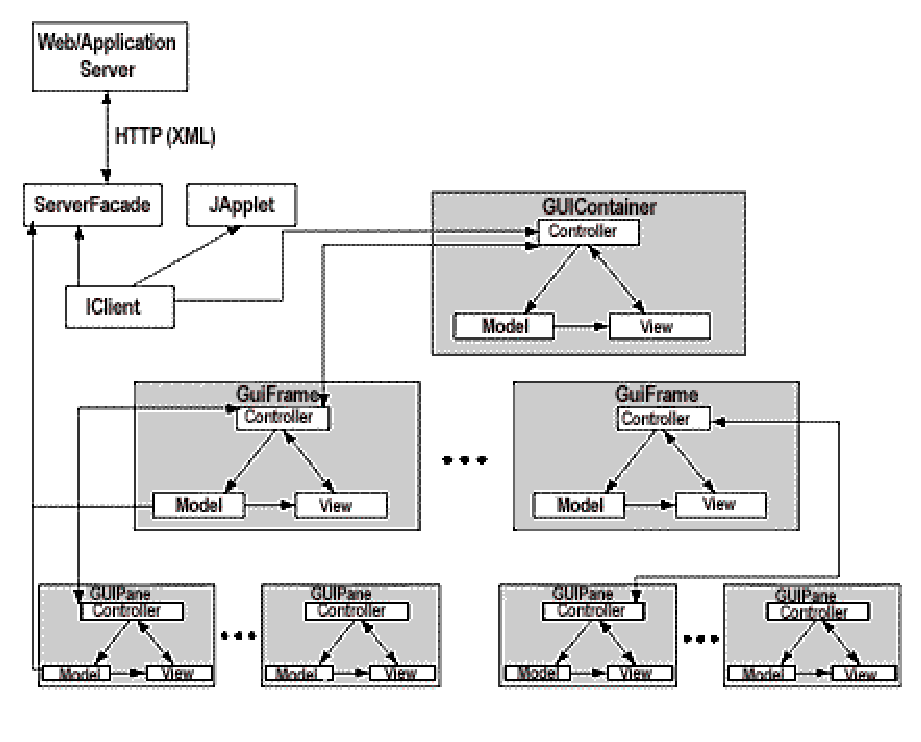
\includegraphics[scale=0.4]{hmvc_client_tier_instance_diagram_cai}
\caption{HMVC Client Tier Instance Diagram \cite{cai}.}
\label{fig:hmvc_client_tier_instance_diagram_cai}
\end{center}
\end{figure}

%
% The extended component lifecycle section.
%
\section{An Extended Component Lifecycle}

Not all components will always need to have a Graphical User Interface (GUI),
as a command line, for example, is often enough to control the component.
Similarly, not all components are based on a specific data model (persistence)
as some components just process direct input without any data storage.

On this point, the question arises, on how to design an application component such
that it has an option, but is not forced to use the complete MVC architecture?

The answer is quite obvious: Let us consider \emph{View} and \emph{Model} to be concerns
of the component! The concerns may be called \emph{Showable} and \emph{Loadable}.

As described before, a component runs through several states of its lifecycle
which is controlled by an outside object, called the \emph{Component Container}.
Depending on the state of several environment variables at runtime, the
container may or may not call certain lifecycle methods of the component.
A GUI-capable component, for example, may have the following lifecycle:

\begin{figure}[ht]
\begin{verbatim}
    configure(c);
    initialize();
    show(v);
    hide(v);
    finalize();
    deconfigure(c);
\end{verbatim}
\caption{Lifecycle of a GUI capable Component.}
\label{fig:lifecycle_of_a_gui_capable_component}
\end{figure}

The source code of [Figure \ref{fig:lifecycle_of_a_gui_capable_component}]
would belong to the component container.
Comparing with the previous example in [Figure \ref{fig:a_component_lifecycle_avalon}],
it can be seen that in [Figure \ref{fig:lifecycle_of_a_gui_capable_component}],
an additional method \emph{show} has been inserted.

Just like the \emph{configure} method gets a configuration object \emph{c} as parameter,
the \emph{show} method gets a view object \emph{v} handed over, which is to be displayed.
Such parameter objects could be created by the container:

\begin{verbatim}
Component c = new ComponentImpl();
View v = new ViewImpl();
c.show(v);
\end{verbatim}

However, most often it is more suitable to let the component create these
parameter objects as they logically belong together:

\begin{verbatim}
Component c = new ComponentImpl();
View v = c.createView();
c.show(v);
\end{verbatim}

This solution has yet another advantage: A view object can be treated as
component itself which means lifecycle methods will have to be called, e.g.:

\begin{verbatim}
View v = new ViewImpl();
v.configure();
v.initialize();
\end{verbatim}

All this is much better encapsulated by a \emph{createView} method in the GUI-capable
component itself, than having the container struggling with it.
If the component shall be based on a specific data model, the corresponding
methods of the \emph{Loadable} concern have to be added to the lifecycle as well:

\begin{verbatim}
Component c = new ComponentImpl();
Model m = c.createModel();
View v = c.createView();
c.load(m);
c.show(v);
\end{verbatim}

The example becomes complete by inserting the code that checks the component
for available conerns:

\begin{verbatim}
Component c = new ComponentImpl();
if (c != null) {
    if (c instanceof Loadable) {
        Model m = c.createModel();
        c.load(m);
    }
    if (c instanceof Showable) {
        View v = c.createView();
        c.show(v);
    }
} else {
    throw new NullPointerException("");
}
\end{verbatim}

Besides the fact that these lifecycle methods can be called or not, there's another advantage:
The container can determine any suitable parameter to hand over to the component.
For example, there may be another view that could be displayed by the component's
\emph{show} method or another data model that might get loaded by \emph{load}.

%
% The resmedlib section.
%
\section{The ResMedLib Framework}

To verify the proposed design, it has been applied and implemented within the
\emph{Res Medicinae} project \cite{resmedicinae}. That is based on the \emph{ResMedLib Framework}
which aims to provide a modular and highly flexible structure to easily implement new components.

Two GUI-capable components have been implemented so far:
The \emph{ResMedicinae} application offering a main window to host sub components (modules)
and the \emph{Record} application meant to become a fully functional \emph{Electronic Health Record (EHR)}. Both modules use a lifecycle similar to the example given above
(Figure \ref{fig:lifecycle_of_a_gui_capable_component}).

The \emph{show} method is implemented by a parent class \emph{AbstractComponent}
[Figure \ref{fig:resmedlib_class_abstractcomponent_in_uml_classdiagram}]
 of the component and can be overridden, of course.
It delegates the task of displaying the view to a \emph{DisplayManager} which can use
Window, Dialog, Frame, InternalFrame or TabPage as possible display. These displays are switchable at runtime.
All this is done by factories, the details of which one can study in the code.

\begin{figure}[ht]
\begin{center}
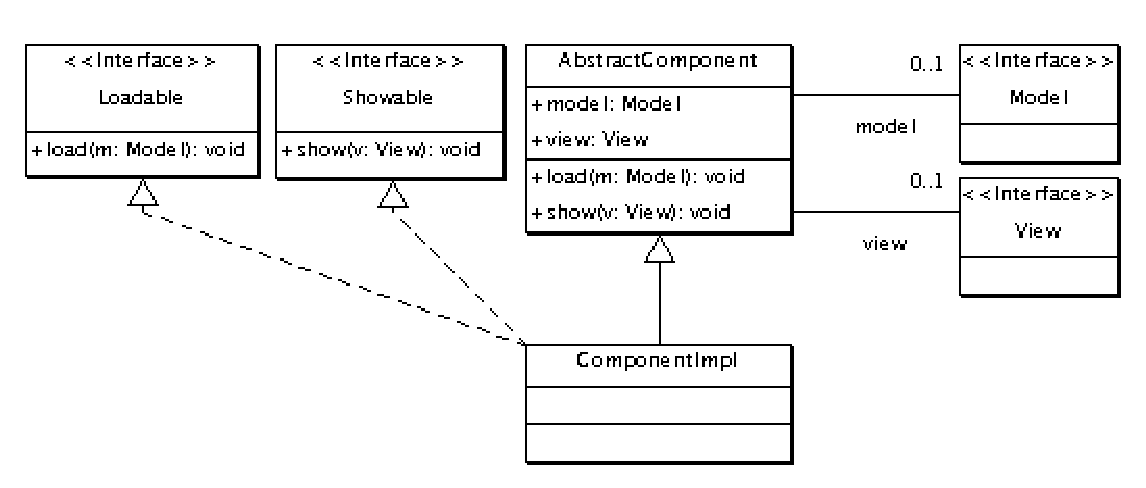
\includegraphics[scale=0.4]{resmedlib_class_abstractcomponent_in_uml_classdiagram}
\caption{ResMedLib class AbstractComponent in UML Class Diagram.}
\label{fig:resmedlib_class_abstractcomponent_in_uml_classdiagram}
\end{center}
\end{figure}

Due to the consistent use of the HMVC design pattern, all application controllers
can be cascaded (Figure \ref{fig:resmedicinae_containing_cascaded_subcomponents}).

\begin{figure}[ht]
\begin{center}
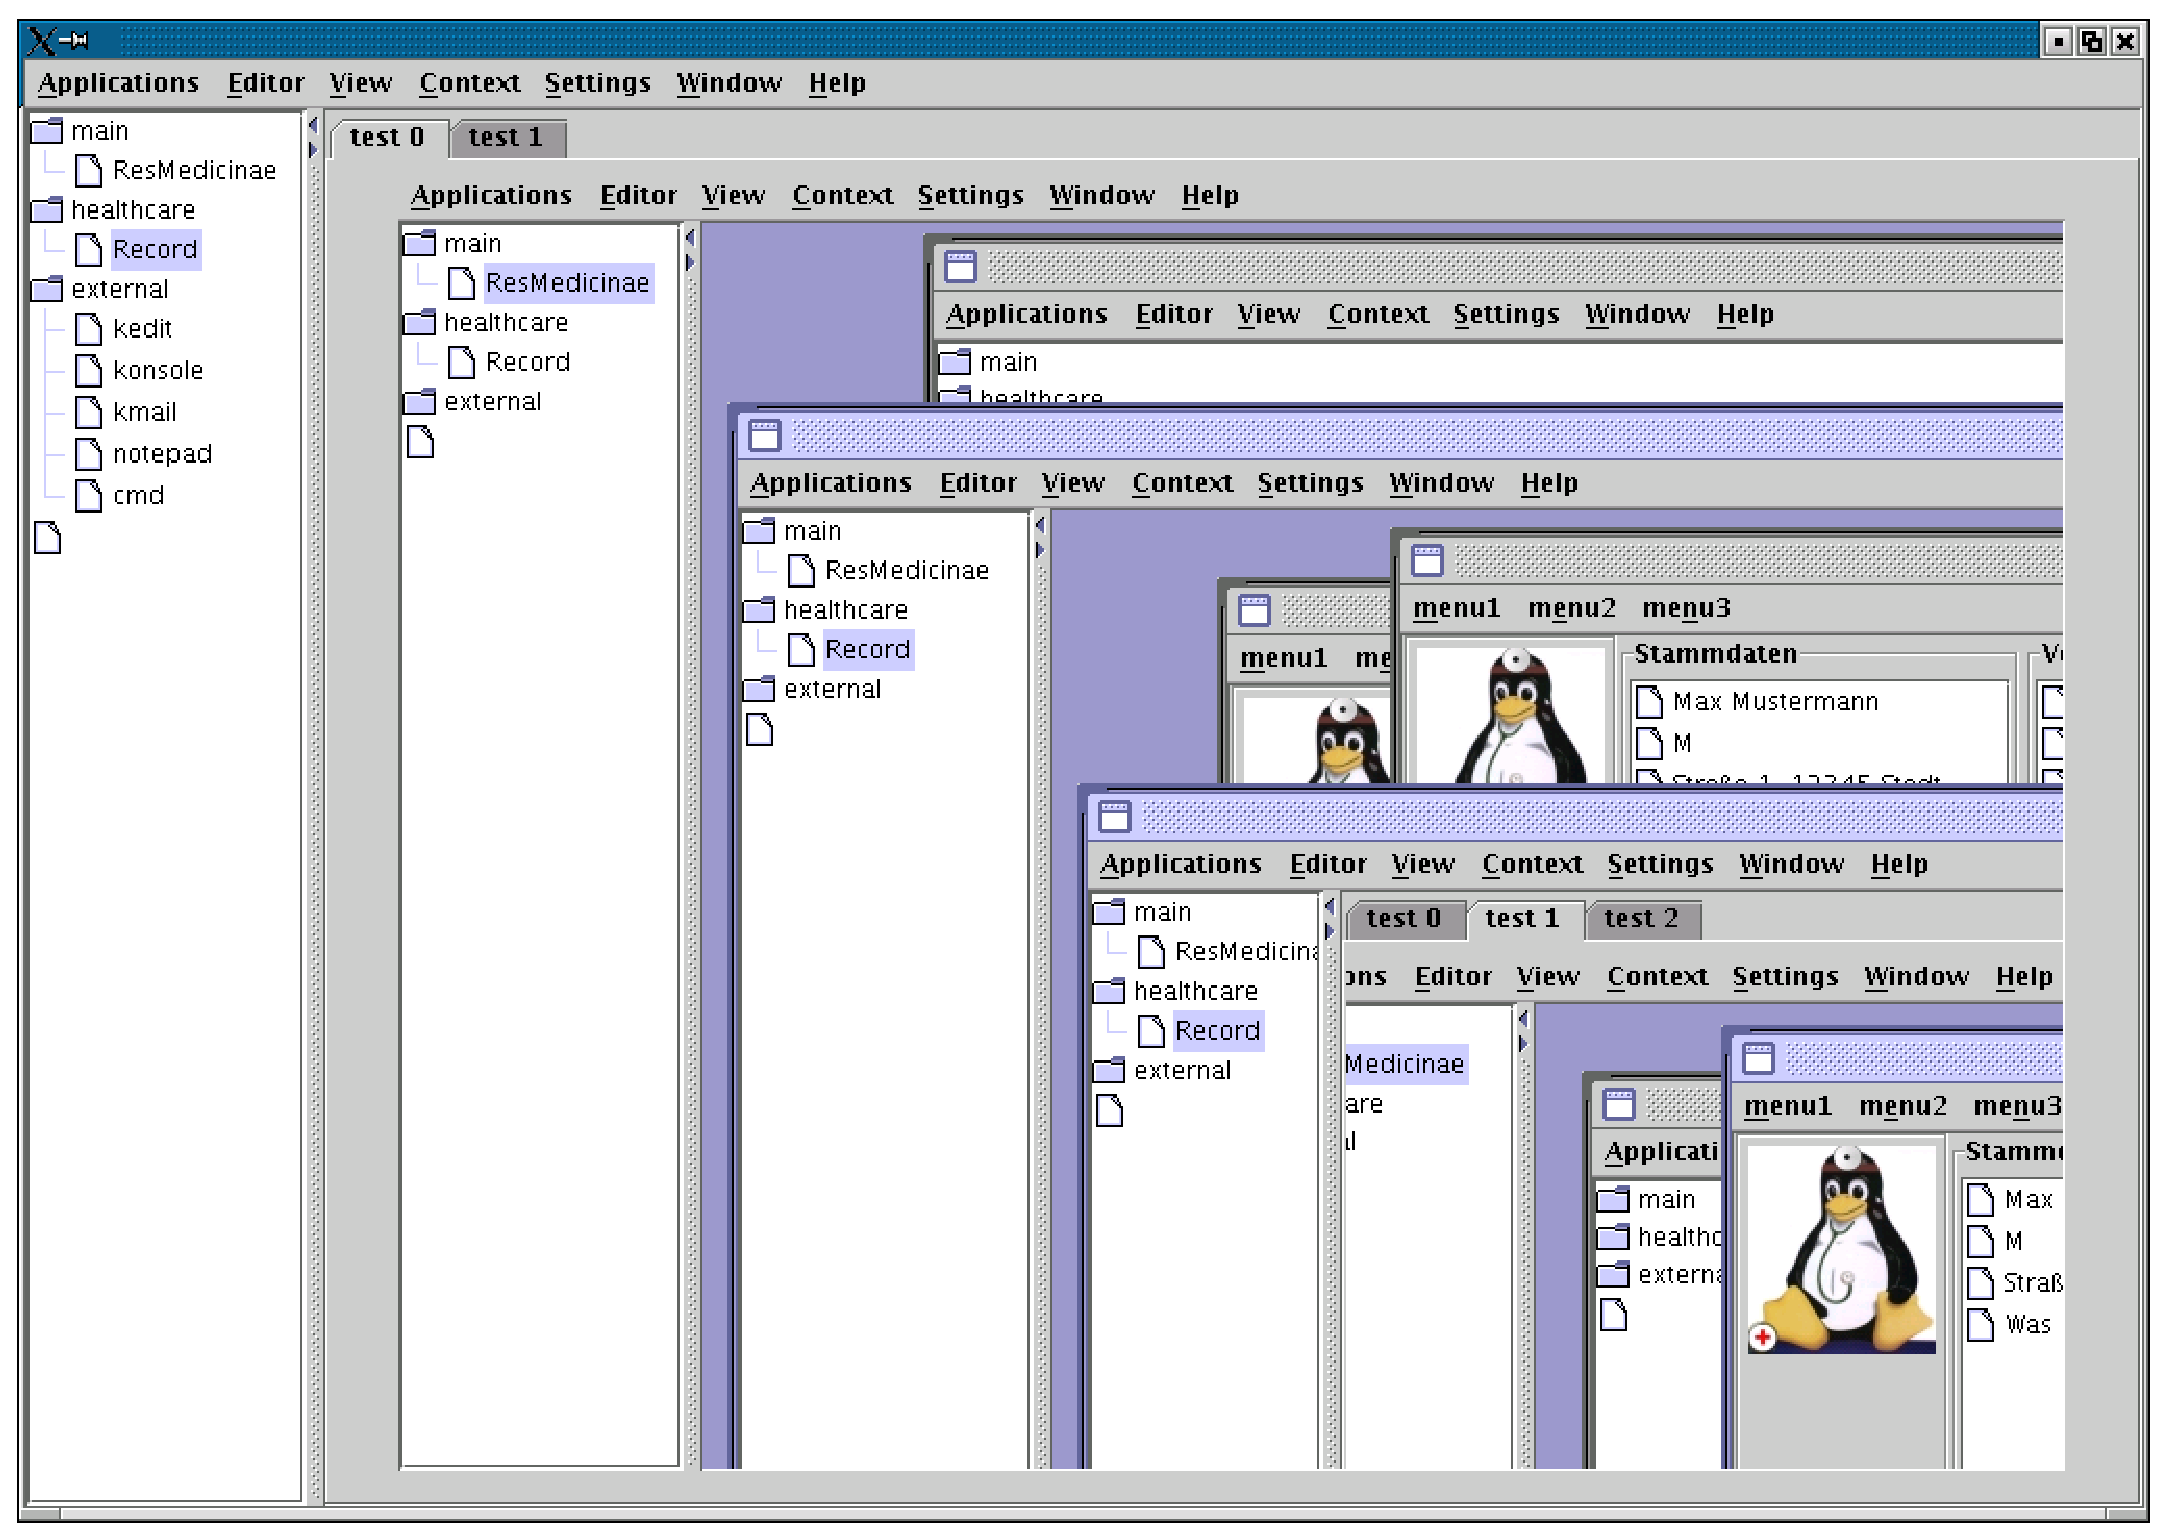
\includegraphics[scale=0.2]{resmedicinae_containing_cascaded_subcomponents}
\caption{Res Medicinae containing cascaded Sub Components.}
\label{fig:resmedicinae_containing_cascaded_subcomponents}
\end{center}
\end{figure}

The \emph{Res Medicinae} project is \emph{Free Software/ Open Source Software (OSS)},
licensed under the \emph{GNU GPL}, i.e. the source code is freely available and extensible,
as well as all documentation and other resources are - as long as derived works are free as well.
Contributions and supporters are always welcome to the project :-)

%
% The summary and future section.
%
\section{Summary and Future}

This article proposes the split-up of view and model of the well-known MVC design pattern
into single concerns. These two, resulting concerns were integrated into a common component lifecycle
of two modules in the \emph{Res Medicinae} project. They have proven to work well and to be highly
flexible due to their clear separation.

Using this advanced architecture, developers are now able to create general components
which offer but do not force the use of a view (GUI) and a model (persistent data storage).
This modular structure allows components to be used in most diverse environments
by simply altering some of their lifecycle calls.

It seems that the use of an aspect-oriented language extension such as \cite{aspectj} can be avoided
by sticking to well-defined concerns/interfaces of a component, just handing over necessary parameters.
However, there's still a lot to figure out in this area. Other useful concerns will have to be identified.
Existing systems are recommended to be refactored and slowly move to CBD/COP with lifecycles,
to achieve higher modularity and flexibility.

%
% The acknowledgements section.
%
\section{Acknowledgements}

My special thanks go to all these brave Enthusiasts of the Open Source Community
who have provided me with a great amount of knowledge through a comprising code base to build on.
I especially would like to mention the contributors of \emph{Res Medicinae} \cite{resmedicinae},
the developers of \emph{Scope} \cite{scope}, of \emph{Apache-Jakarta-Avalon} \cite{jakarta}
and all the other OSS projects.

%
% The about the author section.
%
\section{About the Author}

Christian Heller has studied Electrotechnics/Biomedical Informatics at the Technical University of Ilmenau.
He has worked at several small to large-sized companies, including OWiS (OTW UML tool),
Intershop (e-commerce) and a big German insurance company.
Besides, he is the founder of the Java-based ResMedicinae project
- aiming to implement a Medical Information System -
and active developer of the Open Source Community.
In 2001, he returned to his former University where he plans to earn a doctorate.

%
% Literaturverzeichnis.
%

\label{references_heading}
\bibliographystyle{geralpha}
\bibliography{references}

\end{document}
